%% change beamer theme

\documentclass[
    10pt,
    aspectratio=169,
    xcolor={dvipsnames},
    % hyperref={colorlinks=true,linkcolor=blue,urlcolor=blue}
]{beamer}

\renewcommand{\familydefault}{\rmdefault}

\usetheme{metropolis}

\usepackage{graphicx}
\usepackage{amsmath}
\usepackage{amssymb}
\usepackage{soul}

\newcommand{\presenter}{Meesum Qazalbash}
% \newcommand{\presenter}{Syeda Aliya Fatima Rizvi}

\title{Hempel's Problem}
\author{\presenter}
\date{\today}

\begin{document}
\maketitle

\begin{frame}
    \frametitle{Introduction}
    \textit{Hempel's Problem} was described by \textbf{Carl Gustav Hempel} in an article published in 1945 in the journal \textit{Mind}, int he context of confirmation theory.

    \begin{figure}[h]
        \centering
        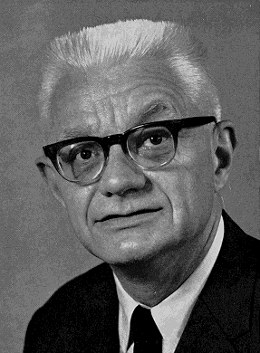
\includegraphics[scale=0.3]{Carl_Gustav_Hempel.jpeg}
        \caption{Carl Gustav Hempel}
    \end{figure}
\end{frame}

\begin{frame}
    \frametitle{Statement}
    \begin{block}{Hempel's Problem}
        \textit{If all ravens are black, then observing a black raven confirms the hypothesis that all ravens are black. But observing a green apple also confirms this  hypothesis, even though apples are not ravens.}
    \end{block}
\end{frame}

\begin{frame}
    \frametitle{Explaination}
    By contrapositive, statement about raven can be written as \ul{\textit{If something is not black, then it is not a raven.}} And apple is not black, so it is not a raven. Hence, it confirms the hypothesis.
\end{frame}

\begin{frame}
    \frametitle{Books Explaination}
    \begin{enumerate}[(1)]
        \item All raven are black [Hypothesis 1]
        \item All non-black objects are non-ravens [Hypothesis 2]
        \item (2) is equivalent to (1) [Contraposition]
        \item The instances that confirm a proposition P also confirms a proposition P* which is equivalent [Premise]
        \item The discovery of a green apple confirms (2) [from (3) and (4)]
        \item \(\therefore\) the discovery of a green apple confirms (1) [from (4) and (5)]
    \end{enumerate}
\end{frame}

\begin{frame}
    \frametitle{Solution I}
    One solution to this problem by simply accepting the conclusion that the discovery of a green apple confirms the hypothesis that all ravens are black.
    \vfill
    But this solution confirms the hypothesis to \textit{infinistimal degree.}
    \vfill
    Which means that the hypothesis is confirmed by the discovery of a green apple, but only to a very small degree.
\end{frame}

\begin{frame}
    \frametitle{Solution II}
    Paul Feyerabend argued that we should only consider negative instances.

    \vfill

    In simple words, he argued that he will not accept it to be true until it is proven to be false.
\end{frame}

\begin{frame}
    \frametitle{Solution III}
    This solution considers Hempel problem and Goodman paradox as a result of unristricted application of inductive logic.
\end{frame}

\begin{frame}
    \frametitle{Conclusion}
    \begin{itemize}
        \item Hempel's problem is a paradox in the philosophy of science.
        \item It was proposed by Carl Gustav Hempel in 1945 to illustrate a problem where inductive logic violates intuition.
        \item The problem is in the counterintuitive nature of confirmation.
        \item There are several solutions to this problem.
        \item The most accepted solution is that the hypothesis is confirmed to a very small degree.
    \end{itemize}
\end{frame}

\begin{frame}
    \frametitle{No Question please}
    \begin{center}
        {\LARGE Questions?}
    \end{center}
\end{frame}

\begin{frame}
    \begin{center}
        {\LARGE Thank You}
    \end{center}
\end{frame}

\end{document}